\section*{Algorytm}
Zadaniem algorytmu w szachach jest znalezienie najlepszego ruchu w danej pozycji poprzez przewidywanie strategii przeciwnika. Słowo "strategia" jest kluczowe, gdyż odnosi się do planowania rozgrywki w przód, która ma na celu osiągnięcie celu w przyszłości, a nie w obecnym ruchu. Do tego celu idealnie nadają się algorytmy drzewiaste, które próbują przewidzieć przyszłość poprzez analizę kombinacji ruchów swoich jak i przeciwnika.

\section*{Drzewo minimax}
Drzewo minimax jest bardzo prostym jak i skutecznym algorytmem do przewidywania ruchów. Prostota polega na stworzeniu kombinacji wszystkich możliwych ruchów i wybranie ścieżki, która prowadzi do najlepszego wyniku. Nazwa wzięła się od tego, że algorytm gra sam ze sobą i wybiera ścieżkę minimalizując wynik przeciwnika równocześnie maksymalizując swój. 


% https://medium.com/@aidenrtracy/the-minimax-algorithm-f6e8e0a1eadb

\begin{figure}[!ht]
\centering
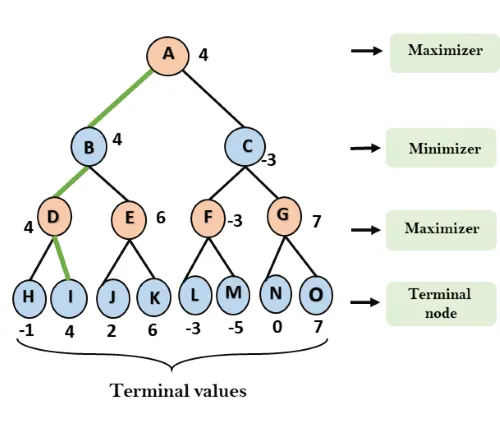
\includegraphics[width=0.4\textwidth]{images/minimax.jpg}
\caption{Drzewo minimax}
\end{figure}

\section*{Drzewo minimax w wersji alpha-beta}
Drzewo minimax w wersji alpha-beta jest zoptymalizowaną wersją algorytmu minimax. Eliminuje ona część gałęzi drzewa, dzięki czemu znacznie szybciej przeszukuje przestrzeń stanów. Jak sama nazwa wskazuje, wprowadza dodatkowo dwie zmienne alpha i beta. Alpha jest maksymalną wartością jaka może pojawić się w maksymalizującym węźle, a beta minimalną wartością jaka może pojawić się w minimalizującym węźle. Jeżeli podczas przeszukiwania drzewa wartość beta będzie mniejsza lub równa alpha to gałąź jest odcinana. Dzięki czemu unikamy niepotrzebnego przeszukiwania gałęzi drzewa, gdyż nie ma sensu sprawdzać ruchów, które nie moga bardziej zminimalizować, bądź zmaksymalizowac wyniku.

Złożoność czasowa minimax wynosi $O(b^d)$, gdzie $b$ to liczba możliwych ruchów w danym stanie, a $d$ to głębokość drzewa. W przypadku zastosowania alpha-beta, złożoność ta może zostać zredukowana do $O(b^{d/2})$ przy najlepszej kolejności ruchów. Możemy zauważyć, że w najlepszym przypadku jesteśmy w stanie stworzyć dwa razy głębsze drzewo.

\begin{figure}[!ht]
\centering
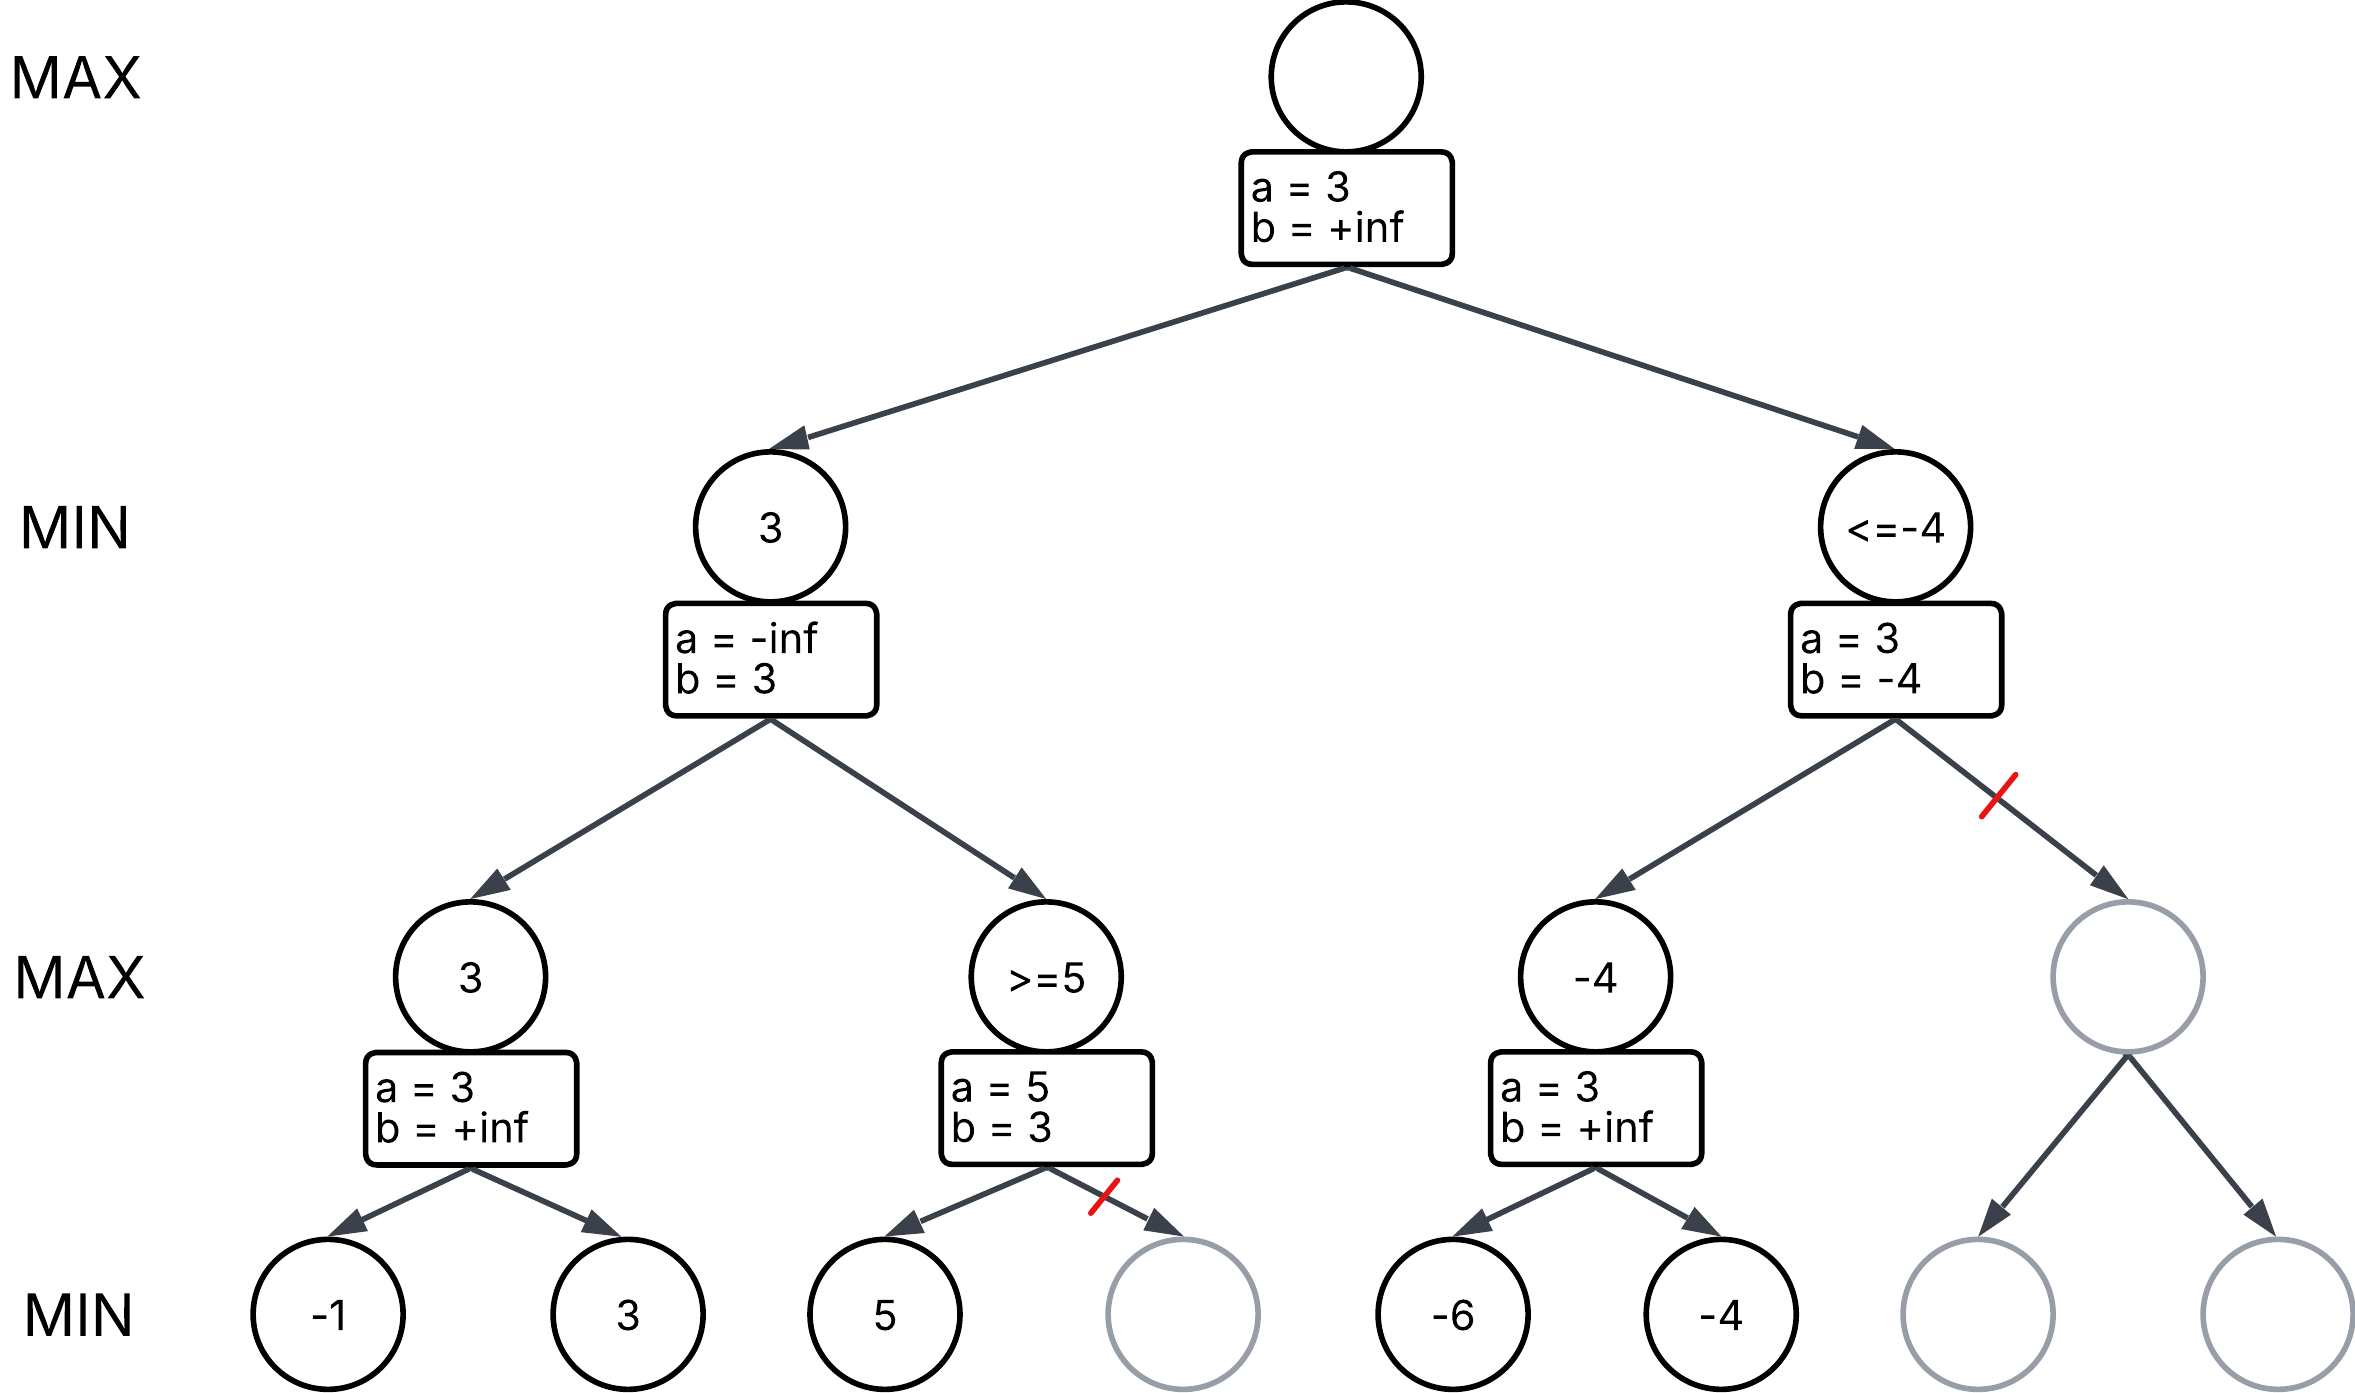
\includegraphics[width=0.6\textwidth]{images/alpha-beta.png}
\caption{Drzewo alpha-beta}
\end{figure}

\section*{Wady drzewa minimax}
Wyżej opisane drzewo minimax jest skuteczne do przewidywania ruchów w grach o małej przestrzeni stanów. W grach o większej złożoności takie jak szachy, zaczynają pojawiać się problemy. Ze względu na ograniczenia pamięciowe jak i czasowe, nie jest możliwe przeszukanie całego drzewa, nawet przy użyciu zoptymalizowanej wersji alpha-beta. Można ograniczyć głębokość drzewa, lecz w przypadku szachów jest to niemożliwe ze względu na brak metody oceniającej planszy w danym stanie. Rozwiązaniem tych problemów jest algorytm Monte Carlo Tree Search.

\section*{Drzewo monte carlo}
Algorytm Monte Carlo Tree Search jest heurystycznym algorytmem przeszukiwania zbioru stanów. Jego największą zaletą jest iteracyjność, dzięki czemu w zależności od dostępnej mocy obliczeniowej (czasu) możemy tworzyć dowolnie duże drzewo i po każdej iteracji jest w stanie zwrócić najlepszy ruch. Dodatkowo w podstawowej wersji nie wymaga skomplikowanej funkcji oceniającej dany stan. Działanie algorytmu opiera się na czterech etapach: selekcji, ekspansji, symulacji oraz wstecznej propagacji.

\begin{figure}[!ht]
\centering
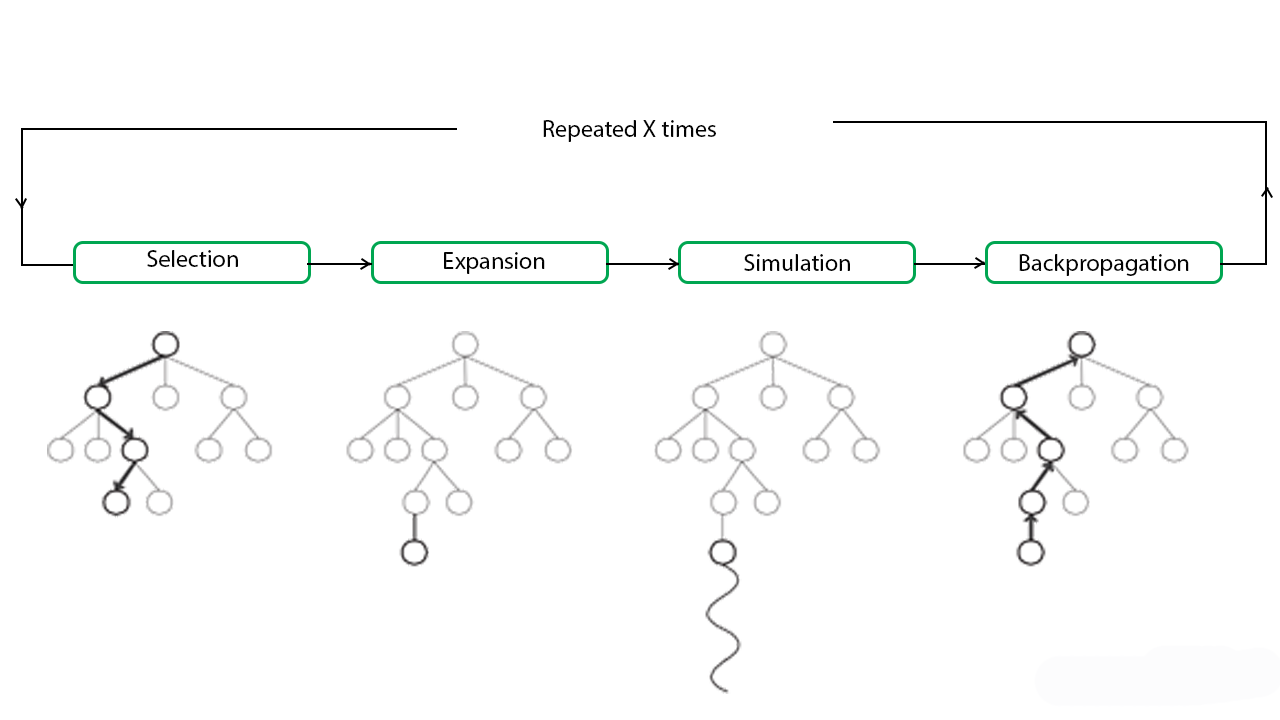
\includegraphics[width=0.6\textwidth]{images/mcts_sections.png}
\caption{Etapy algorytmu Monte Carlo Tree Search}
\end{figure}

\section{Selekcja}
Etap selekcji, jak sama nazwa wskazuje wybiera najbardziej obiecujący liść do dalszego rozwoju drzewa. Liść jest rozumiany jako węzeł, który nie został jeszcze całkowicie rozwinięty, czyli nie posiada jeszcze wszystkich swoich dzieci.
Dany węzeł jest wybierany na podstawie maksymalizacji funkcji UCT:

\begin{equation}
\operatorname{UCT}(s,a) \,=\, \widehat{Q}(s,a) \, + \, c\, \sqrt{\frac{\ln(N(s))}{N(s,a)}},\,
\quad
\widehat{Q}(s,a) \,=\, \dfrac{W(s,a)}{N(s,a)}\,
\end{equation}

\noindent gdzie:
\begin{description}
  \item[$N(s)$] - liczba odwiedzin stanu $s$
  \item[$N(s,a)$] - liczba odwiedzeń akcji $a$ w stanie $s$
  \item[$W(s,a)$] - wartość sumy nagród akcji $a$ w stanie $s$
  \item[$c$] - współczynnik eksploracji
\end{description}

\hspace{1cm}

Wzór ten składa się z sumy dwóch części. Pierwsza z nich $\widehat{Q}(s,a)$ odpowiada za eksploatację, czyli wybór węzła, który jak dotąd osiągnął najlepszy wynik. Druga część $c\, \sqrt{\frac{\ln(n_s)}{n_{s,a}}}$ skupia się na eksploracji, czyli wyborze węzła, który był rzadziej odwiedzany. Na poniżyszm wykresie możemy zauważyć, że część ta znacznie bardziej faworyzuje mniejszą liczbę odwiedzin $n_{s,a}$, ponadto użycie logarytmu naturalnego sprawia, że zmiana liczby odwiedzin węzła rodzica nie powoduje nagłych zmian w wartości eksploracji. Współczynnik $c$ we wzorze pozwala nam dostosować balans między eksploracją, a eksploatacją.

\begin{figure}[!t]
\centering
\begin{tikzpicture}
\begin{axis} [
    xlabel={Liczba odwiedzin węzła $n_{s,a}$},
    ylabel={Wartość eksploracji},
    grid=major,
    width=10cm,
    height=6cm,
    domain=1:30,
    samples=200
]
\addplot[blue, thick] {sqrt(ln(50)/x)};
\legend{$\sqrt{\frac{\ln 50}{n_{s,a}}}$}
\end{axis}
\end{tikzpicture}
\caption{Składnik eksploracji $\sqrt{\frac{\ln(n_s)}{n_{s,a}}}$ dla $n_s=50$}
\label{fig:uct-exploration}
\end{figure}

\section{Ekspansja}
Etap ekspansji ma za zadanie rozwijać drzewo poprzez dodanie jednego nowego węzła do wybranego liścia. Nowy węzeł jest wybierany losowo spośród wszystkich możliwych ruchów, które nie zostały jeszcze dodane do drzewa.

\section{Symulacja}
Etap symulacji polega na przeprowadzeniu symulacji rozgrywki \textbf{od} nowo dodanego węzła do końca gry w sposób losowy. W przypadku szachów oznacza to wykonywanie losowych ruchów aż do osiągnięcia stanu końcowego: mat, pat, remis.

\section{Wsteczna propagacja}
Etap wstecznej propagacji polega na propagowaniu wyniku symulacji w górę drzewa. Aktualizowane są wszystkie węzły od nowo dodanego węzła do korzenia. W każdym z tych węzłów zwiększana jest liczba odwiedzin, oraz sam wynik gry.